\documentclass[letterpaper,10pt]{article}

\usepackage{latexsym}
\usepackage[empty]{fullpage}
\usepackage{titlesec}
\usepackage{marvosym}
\usepackage[usenames,dvipsnames]{color}
\usepackage{verbatim}
\usepackage{enumitem}
\usepackage[hidelinks]{hyperref}
\usepackage{fancyhdr}
\usepackage[english]{babel}
\usepackage{tabularx}
\usepackage{geometry}
\usepackage{graphicx}
\graphicspath{{assets/}{../assets/}}

\geometry{top=0.3in, bottom=0.3in, left=0.45in, right=0.45in}

\pagestyle{fancy}
\fancyhf{}
\fancyfoot{}
\renewcommand{\headrulewidth}{0pt}
\renewcommand{\footrulewidth}{0pt}

\urlstyle{same}
\raggedbottom
\raggedright
\setlength{\tabcolsep}{0in}

\titleformat{\section}{
  \vspace{-6pt}\scshape\raggedright\large\bfseries
}{}{0em}{}[\color{black}\titlerule \vspace{-4pt}]

\newcommand{\resumeItem}[1]{
  \item\small{#1 \vspace{-1.5pt}}
}

\newcommand{\resumeSubheading}[4]{
  \vspace{-2pt}\item
    \begin{tabular*}{1.0\textwidth}[t]{l@{\extracolsep{\fill}}r}
      \textbf{#1} & \textbf{\small #2} \\
      \textit{\small#3} & \textit{\small #4} \\
    \end{tabular*}\vspace{-6pt}
}

\newcommand{\resumeProjectHeading}[2]{
    \item
    \begin{tabular*}{1.0\textwidth}{l@{\extracolsep{\fill}}r}
      \small#1 & \textbf{\small #2}\\
    \end{tabular*}\vspace{-4pt}
}

\renewcommand\labelitemi{$\vcenter{\hbox{\tiny$\bullet$}}$}
\newcommand{\resumeSubHeadingListStart}{\begin{itemize}[leftmargin=0.0in, label={}]}
\newcommand{\resumeSubHeadingListEnd}{\end{itemize}}
\newcommand{\resumeItemListStart}{\begin{itemize}[leftmargin=0.15in, itemsep=-1pt, topsep=0pt]}
\newcommand{\resumeItemListEnd}{\end{itemize}\vspace{-4pt}}

\begin{document}

%----------HEADING----------
\begin{tabularx}{\textwidth}{@{}X c@{}}
  \begin{minipage}[c]{\linewidth}
    \textbf{\Huge Lakshya Singhi} \\[8pt]
    \href{mailto:lakshyasinghi16@gmail.com}{lakshyasinghi16@gmail.com} \quad +91 93304 60428 \\[5pt]
    \href{https://github.com/lakshya0511}{\underline{GitHub}} $|$
    \href{https://www.linkedin.com/in/lakshya-singhi-a3108736a/}{\underline{LinkedIn}}
  \end{minipage}
  &
  \begin{minipage}[c]{0.95in}
    \raggedleft
    \setlength{\fboxsep}{0pt}%
    \frame{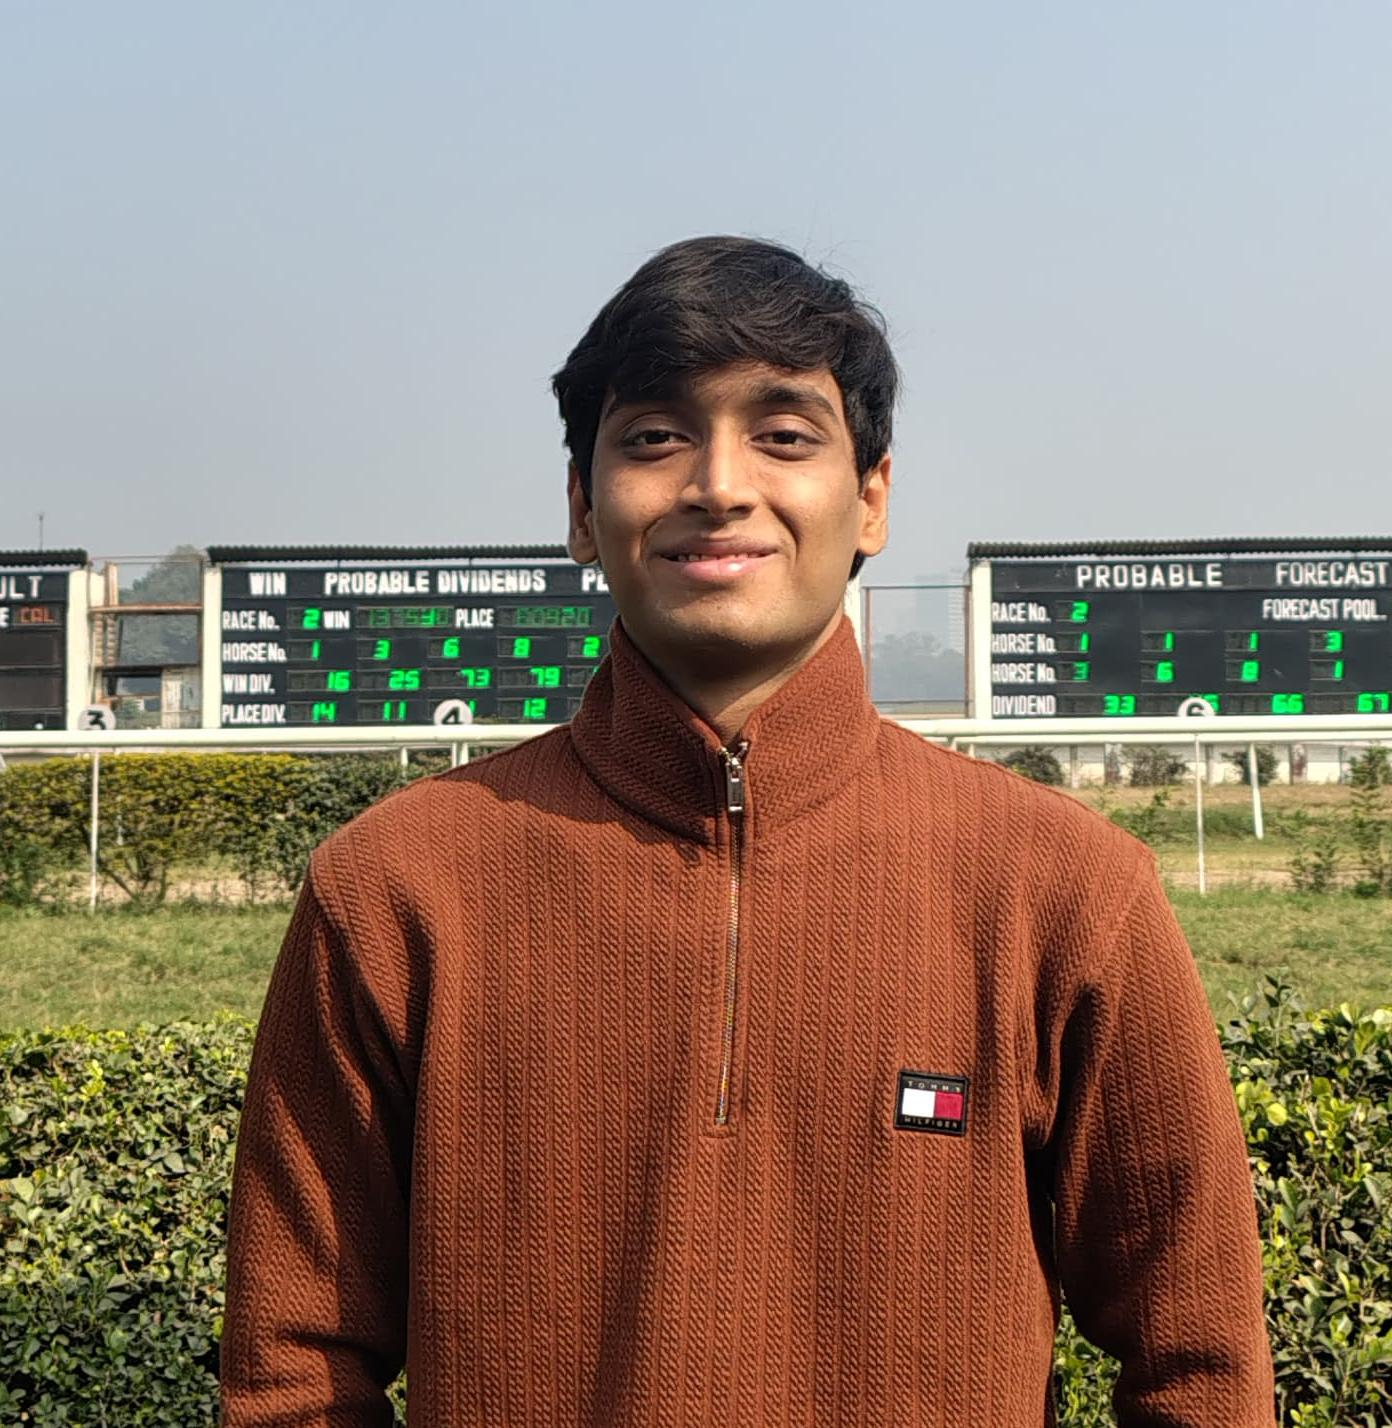
\includegraphics[width=0.75in,height=0.9in]{image.jpeg}}
  \end{minipage}
\\
\end{tabularx}

%-----------EDUCATION-----------
\section{Education}
  \resumeSubHeadingListStart
    \resumeSubheading
      {Manipal Institute of Technology $|$ \normalfont\small GPA: 8.54/10}{Manipal, Karnataka}
      {Bachelor's of Technology in Information Technology}{August 2024 -- May 2028}
      \vspace{2pt}
    \resumeItemListStart
      \resumeItem{Relevant Coursework: Data Structures \& Algorithms, Object-Oriented Programming, 
      Operating Systems, Database Management Systems,  Computer Networks, System Design, Data Analytics}
    \resumeItemListEnd
  \resumeSubHeadingListEnd

%-----------EXPERIENCE-----------
\section{Experience}
  \resumeSubHeadingListStart

    \resumeSubheading
      {EaseOps}{June 2026 -- July 2026}
      {Frontend Developer Intern}{}
      \vspace{1pt}
    \resumeItemListStart
      \resumeItem{Engineered the Asset Management, Reminders, and Leaderboard modules for an enterprise Hospital Management System, delivering cross-platform screens in Flutter (mobile and web) from product requirements to production.}
      \resumeItem{Developed interactive dashboards that surfaced asset and activity metrics, integrating the UI with backend REST APIs for data fetching, state management, and error handling.}
      \resumeItem{Collaborated cross-functionally with backend engineers to integrate frontend components with backend services, resolving data-mapping and pagination defects that were breaking list and dashboard views in production.}
      \resumeItem{Debugged and resolved client-reported production defects by inspecting API responses and application logs to trace root causes, reducing recurring frontend-backend synchronization issues.}
    \resumeItemListEnd

    \vspace{2pt}
    \resumeSubheading
      {Glo School (Gyan Saarthi Education Pvt Ltd)}{January 2026 -- April 2026}
      {Software Development Intern}{}
      \vspace{1pt}
    \resumeItemListStart
      \resumeItem{Built a Flutter and Firebase web application for kindergarten teachers, enabling daily task management, lesson planning, instructional workflows, and student feedback through a centralized dashboard.}
      \resumeItem{Designed Firestore data models and implemented application features with real-time synchronization, collaborating in an Agile team to deliver, test, and debug features across the full application stack.   
         (\href{https://drive.google.com/file/d/12q9jS7Z0fGUwRlL-mA-XL8nYIhbcy4dA/view}{\underline{View LOR}})}
    \resumeItemListEnd

  \resumeSubHeadingListEnd

%-----------PROJECTS-----------
\section{Projects}
  \resumeSubHeadingListStart

    \resumeProjectHeading
      {\textbf{Dhan Mitra -- Fintech Simulation Platform} $|$ \textit{\small Flutter, Firebase} $|$ \href{https://github.com/lakshya0511/dhan_mitra}{\underline{GitHub}} $|$ \href{https://dhanmitra-26.web.app/}{\underline{Live Demo}}}{January 2026 -- Present}
    \resumeItemListStart
      \resumeItem{Developed a cross-platform fintech learning platform using Flutter and Firebase, combining multilingual investment courses, scenario-based quizzes, and virtual trading to help users learn investing through hands-on practice.}
     \resumeItem{Implemented SIP, SWP, and stock-market simulation engines with Firestore, alongside AI-generated personalized quiz feedback, authentication, wallet management, and real-time portfolio synchronization.}
     \resumeItem{Architected the application using modular state management and reusable components, applying object-oriented design principles to support scalable feature development and future financial learning modules.}
    \resumeItemListEnd

    \vspace{3pt}
    \resumeProjectHeading
      {\textbf{Revels OM Portal} $|$ \textit{\small React, Node.js, PostgreSQL}}{December 2025 -- January 2026}
    \resumeItemListStart
      \resumeItem{Built a scalable backend for a room booking portal serving 700+ outstation participants using Node.js and PostgreSQL, implementing normalized database schemas and REST APIs for room allocation and booking management.}
      \resumeItem{Implemented role-based authorization and booking workflows that sustained peak concurrent registration traffic without double-booking slots.}
    \resumeItemListEnd

    \vspace{3pt}
    \resumeProjectHeading
      {\textbf{Xuberance Event Management App} $|$ \textit{\small Flutter, Firebase}}{August 2022 -- October 2022}
    \resumeItemListStart
      \resumeItem{Built a cross-platform event app in Flutter and Firebase for 200+ participants, supporting event registration and live schedule updates.}
      \resumeItem{Implemented Firebase Authentication, Firestore integration, and push notifications to keep participants updated during the event.}
    \resumeItemListEnd
    

  \resumeSubHeadingListEnd

%-----------LEADERSHIP-----------
\section{Leadership}
  \resumeSubHeadingListStart

    \resumeSubheading
      {Development Team}{December 2025 -- Present}
      {Student Council, MIT Manipal}{}
      \vspace{1pt}
    \resumeItemListStart
      \resumeItem{Develop backend systems and web portals for college fests, implementing REST APIs and features to streamline event operations.}
      \resumeItem{Built a Club Management System with role-based authentication, multi-level approval workflows, and REST APIs used to coordinate club activities across campus.}
    \resumeItemListEnd
    \vspace{2pt}
    \resumeSubheading
      {App Dev Head}{July 2025 -- Present}
      {ACM Manipal}{}
      \vspace{1pt}
    \resumeItemListStart
      \resumeItem{Lead the App Development domain by organizing technical sessions, mentoring members, and coordinating development activities.}
    \resumeItemListEnd
  \resumeSubHeadingListEnd

%-----------SKILLS-----------
\section{Technical Skills}
\begin{itemize}[leftmargin=0.15in, label={}, itemsep=0pt]
  \small{\item{
    \textbf{Languages:} Java, Python, C, JavaScript, Dart, SQL \\
    \textbf{Frameworks \& Libraries:} React, Next.js, Node.js, Flutter \\
    \textbf{Backend \& Databases:} REST APIs, Firebase, PostgreSQL, Firestore, Database Design, Backend Development \\
    \textbf{Core CS:} Data Structures \& Algorithms, Object-Oriented Programming, Operating Systems, DBMS, Computer Networks, System Design \\
    \textbf{Developer Tools:} Git, GitHub, Postman, Figma, Linear
  }}
\end{itemize}

\end{document}